\documentclass[12pt,a4paper, bibliography=totocnumbered]{scrreprt}

\usepackage[ngerman]{babel}
\usepackage[utf8]{inputenc}
\usepackage[T1]{fontenc}
\usepackage{times}
\usepackage{booktabs}
\usepackage{tabularx}
\usepackage{geometry}
\usepackage{graphicx}
\usepackage{xcolor}
\usepackage{amssymb}
\usepackage{scrhack} % get rid of warning in combination with listings package
\usepackage{listings}
\usepackage{lipsum}
\usepackage{pgfgantt}
\usepackage[
	hidelinks,
	plainpages=false,
	colorlinks=true,
	linkcolor=black,
	filecolor=black,
	urlcolor=black,
	citecolor=black,
	bookmarksnumbered=true,
	bookmarksopen=true,
	bookmarksopenlevel=4
]{hyperref}

%this can be used for syntax highlighting of java code
% predefined colors for source-code
\definecolor{darkred}{rgb}{.6,0,0}
\definecolor{darkmagenta}{rgb}{.6,0,.6}
\definecolor{darkgreen}{rgb}{0,.6,0}
\definecolor{turqoise}{cmyk}{0.9,0,0.2,0.3}

% setup of code-evironments
\lstloadlanguages{Java,XML}

% Hacked Java-environment to support Annotations with different color
% usage: 
% \begin{java} 
%   your code 
% \end{java}
\lstnewenvironment{java}[1][]{%
\vspace{0.1em}\fontfamily{pcr}\selectfont
	\lstset{
	  language=Java,
	  basicstyle=\scriptsize,	  
 	  showspaces=false,
	  showtabs=false,
	  columns=fixed,
	  numbers=left,
	  frame=single,
	  numberstyle=\tiny,
	  breaklines=false,
	  showstringspaces=false,
	  tabsize=3,
	  keywordsprefix={@}, % only available in first keywords-list
	  keywords=[1]{}, % delete all java-keywords in first list
	  keywords=[2] {abstract,assert,boolean,break,byte,case,catch,char,class,const,continue,default,do,double,else,enum,extends,false,final,finally,float,for,goto,if,implements,import,instanceof,int,interface,long,native,new,null,package,private,protected,public,return,short,static,strictfp,super,switch,synchronized,this,throw,throws,transient,true,try,void,volatile,while}, % put them into the second list
	  commentstyle=\itshape\color{darkgreen},
	  keywordstyle=[1]\color{turqoise}, % print all annotations in turqoise
	  keywordstyle=[2]\bfseries\color{darkmagenta}, % print all java-keywords in eclipse-color
	  stringstyle=\color{blue},
	  #1
	}
}
{\normalfont\selectfont}

% Defines an XML-Code-Environment
% usage: 
% \begin{xml} 
%   your code 
% \end{xml}
\lstnewenvironment{xml}{
\vspace{0.1em}\fontfamily{pcr}\selectfont
	\lstset{
	  language=XML,
		basicstyle=\scriptsize,
	  commentstyle=\itshape\color{darkgreen},
	  keywordstyle=\bfseries\color{darkred},
	  stringstyle=\tt\color{blue},
	  showspaces=false,
	  showtabs=false,
	  columns=fixed,
	  numbers=none,
	  frame=single,
	  numberstyle=\tiny,
	  breaklines=false,
	  showstringspaces=false,
	  tabsize=3,
	  moredelim=**[s][\bfseries\color{darkred}]{<}{>},
	}
}
{\normalfont\selectfont}


%%%%%%%%%%%%%%%%%%%%%%%%%%%%%%%%%%%%%%%%%%%%%%%%%%%%%%%%%%%%%%%%%%%%%%%%%%%%
\begin{document}

%%%%%%%%%%%%%%%%%%%%%%%%%%%%%%%%%%%%%%%%%%%%%%%%%%%%%%%%%%%%%%%%%%%%%%%%%%%%
%%%%%%%%%%%%%%%%%%%%%%%%%%%%%%%%%%%%%%%%%%%%%%%%%%%%%%%%%%%%%%%%%%%%%%%%%%%%
% Cover Page
%%%%%%%%%%%%%%%%%%%%%%%%%%%%%%%%%%%%%%%%%%%%%%%%%%%%%%%%%%%%%%%%%%%%%%%%%%%%
\renewcommand{\title}{NVD-Schwachstellendatenbank}
\pagenumbering{Alph}
\thispagestyle{empty}
\begin{titlepage}
\begin{center}

\begin{tabularx}{\textwidth}{p{.28\textwidth}X@{\extracolsep\fill}p{.25\textwidth}}
\parbox[c]{\hsize}{
\includegraphics[scale=0.25]{figures/tu-logo}} & 
Technische Universit\"at Berlin\hfill & 
\parbox[c]{\hsize}{
\includegraphics[scale=0.3]{figures/dai-logo}} 
\end{tabularx}

\rule{\textwidth}{0.4pt}

\vspace{7em}
\textbf{\huge\title}
\vspace{7em}

\begin{large}\textbf{Projektbericht}\end{large} \\
AOT-Praktikum Intelligente Softwaresysteme\\
Fakult\"at IV Elektrotechnik und Informatik \\
Technische Universit\"at Berlin \\[4em]
\textbf{Gruppe 1} \\

\vfill

\begin{tabular}{ll} Betreuer: \\ \end{tabular} \\
\vspace{2em}
\textbf{SoSe 2018} \\

%\vfill
\end{center}
\end{titlepage}

\pagenumbering{roman}
\chapter*{Abstract (Patrick)}
% Folgende Infos aus dem Leitfaden für wissenschaftliche  Arbeiten der TU Berlin:
% https://www.proscience.tu-berlin.de/fileadmin/fg15/archiv_berichte_reporting/2013/assisthesis_studierendenversion1.pdf
% Kurzfassung, Zusammenfassung: 
% 1.) Das Abstract verrät mir, ob die Arbeit für mich interessant ist.
% 2.) Das Abstract ist allein verständlich, ohne die gesamte Arbeit zu lesen.
% 3.) Der Aufbau gleicht dem des Originaltextes:
% Zitat ASSIS Thesis: 
% „Auskunft über das behandelte Gebiet, Zielsetzungen, Hypothesen, Methoden, Ergebnisse und Schlußfolgerungen der im Originaldokument enthaltenen Überlegungen und Darstellungen, einschließlich der Fakten und Daten. [DIN 1426, S. 3]
Die Relevanz neuer Sicherheitsmechanismen in modernen IT-Infrastruktur Systemen steht immer öfter im Mittelpunkt, wie Angriffe auf große Unternehmen in den letzten Jahren gezeigt haben. Die National Vulnerability Database (NVD) stellt eine Datenbank zur Verfügung, die sicherheitsrelevante Informationen zu IT-Bezogenen Schwachstellen bereit stellt. Ziel der vorliegenden Arbeit ist es, diese Informationen übersichtlich, benutzerfreundlich aufzubereiten und zur Verfügung zu stellen. Es stellt sich heraus, dass die Umsetzung des Projektes mit Spring und MongoDB eine optimale Methode bietet, dem Entwurfsmuster Model View Control (MVC) nachzukommen. Mit Projektmanagement-Methoden wie die Nutzung eines Gantt-Diagramms und der Anwendung von SCRUM für die agile Softwareentwicklung ist es gelungen, die Informationen der NVD aufzubereiten und das Projekt in der geplanten Zeit umzusetzen. Die Planung und Entwicklung innerhalb des Teams und wöchentliche Meetings führen zu einem Ergebnis, dass sämtliche Anforderungen erfüllt und für zukünftige Projekte, wie beispielsweise Applikationen zur Überwachung von IT-Netzwerken, eingesetzt werden kann.

\tableofcontents
\clearpage
\pagenumbering{arabic}

%%%%%%%%%%%%%%%%%%%%%%%%%%%%%%%%%%%%%%%%%%%%%%%%%%%%%%%%%%%%%%%%%%%%%%%%%%%%
% Main content
%%%%%%%%%%%%%%%%%%%%%%%%%%%%%%%%%%%%%%%%%%%%%%%%%%%%%%%%%%%%%%%%%%%%%%%%%%%%
\chapter{Motivation (David)}
Software ist im heutigen digitalen Zeitalter das Fundament, auf dem die Wirtschaft und mittlerweile auch die Gesellschaft basiert. Immer umfangreichere Software-Lösungen finden in der Industrie, aber auch in kapitalintensiven und sicherheitskritischen Bereichen Anwendung \cite{Belli1998MethodenSoftware}. Die Komplexität die bei der Entwicklung derartiger Systeme bewältigt werden muss, stellt zunehmend eine Herausforderung für das Projekt- und Entwicklungsmanagement dar. Die einhergehende Fehleranfälligkeit von komplexen Software-Systemen kann dabei ein hohes Gefahrenpotenzial implizieren. Je nach dem, wo die Software eingesetzt wird, können Software-Fehler neben großen wirtschaftlichen Schäden (zum Beispiel im Bereich des Bankwesens) auch zu Gefahren für Leib und Leben von Menschen führen. So ist die Zuverlässigkeit und Korrektheit von in Passagierflugzeuge eingesetzter Software essentiell für einen sicheren Transport der Passagiere.
\\

Im Allgemeinen können vorhandene Softwarefehler unter bestimmten Bedingungen, aber auch durch bewusstes Verursachen (Provozieren der verantwortlichen Bedingungen) durch Dritte ausgelöst werden. In diesem Kontext tritt das Wort \glqq Schwachstelle\grqq{} (oder auch \glqq Sicherheitslücke\grqq{}) in Erscheinung. Beide Begriffe definieren den Zustand eines Systems, welches durch einen bestimmten Angriff manipuliert oder beschädigt werden kann. Unter dem Begriff Angriff ist in diesem Kontext das mutwillige Ausnutzen beziehungsweise Auslösen eines Software-Fehlers zu verstehen \cite{Al-Fedaghi2010System-basedVulnerability}. Auf diese Weise können beispielsweise Authentifizierungs- und Authorisierungsmechanismen umgangen werden, um sich unberechtigten Zugang zu fremden Computer-Systemen und Netzwerken zu verschaffen. Die Erkennung und Verhinderung von derartigen Angriffen wird in vielen Forschungsarbeiten thematisiert, wie zum Beispiel in dem Buch von Viega und McGraw zur Vermeidung von Sicherheitsproblemen während der Entwicklung neuer Software \cite{Viega2001BuildingWay}.
\\

Da aber auch aktuelle und weit verbreitete Software-Systeme immer wieder von Schwachstellen betroffen sind, ist eine schnelle Behebung dieser, sowie die sofortige Aufklärung der Nutzer enorm wichtig. Für diesen Zweck existieren viele verschiedene Plattformen beziehungsweise Datenbanken, die Informationen zu aktuellen beziehungsweise neu entdeckten Schwachstellen standardisiert speichern und so betroffene Personen und Unternehmen einen schnellen Zugriff zu für sie relevante Daten ermöglichen \cite{Mell2006CommonSystem}.

%Der folgende Projektbericht stellt die Umsetzung einer Plattform dar, auf der Informationen zu Schwachstellen speichert und diese durch verschiedene Such- und Filterfunktionalitäten zur Verfügung stellt. Dabei werden alle Informationen von der National Vulnerability Database (NVD) importiert.

\chapter{Related Work (David)}
Wie aktuelle Statistiken vom Bundesamt für Informationssicherheit (BSI) zeigen, nimmt die Anzahl der Angriffe gegen IT-Systeme ständig zu \cite{furSicherheitinderInformationstechnikDie2017}. Dementsprechend gewannen auch Plattformen beziehungsweise Datenbanken, die sicherheitsrelevante Informationen zu aktuellen Bedrohungen und Handlungsempfehlungen zur Verfügung stellen an Bedeutung. Einrichtungen, wie zum Beispiel das dem \glqq US-CERT\grqq{}  zugehörigen \glqq National Cybersecurity and Communications Integration Center\grqq{} (NCCIC) \cite{NationalSecurity} informiert mit Hilfe von Warnungen, Analysen und Berichten über die aktuelle Gefährdungslage und stellt Hinweise und Ratschläge für Betroffene zur Verfügung. Eine vergleichbare Rolle hat das BSI in Deutschland.
\\

Die genannten Einrichtungen referenzieren dabei auf konkrete Schwachstellen, die durch CVE-Kennungen eindeutig identifizierbar sind. CVE steht hierbei für \glqq Common Vulnerabilities and Exposures\grqq{}. Es handelt sich hierbei um ein Industriestandard, dessen Ziel die Einführung einer einheitlichen Namenskonvention für Schwachstellen in Computersystemen ist \cite{Mell2006CommonSystemb}. Neben CVE sind weitere Standards entstanden, um Eigenschaften beziehungsweise Merkmale von Schwachstellen eindeutig beschreiben zu können. So kann beispielsweise der Schweregrad einer möglichen oder tatsächlichen Schwachstelle durch den \glqq Common Vulnerability Scoring System\grqq{} (CVSS) Standard bewertet werden  \cite{Mell2006CommonSystemb}. Neben dem weit verbreiteten CVSS Standard existiert auch \glqq Common Weakness Scoring System\grqq{} (CWSS), der ebenfalls zur Priorisierung und Bewertung von Sicherheitslücken eingesetzt werden kann. Ein weiterer Standard der im diesem Kontext genannt werden muss, ist \glqq Common Weakness Enumeration\grqq{} (CWE). Mit diesem werden verschiedene Typen beziehungsweise Varianten von Schwachstellen definiert \cite{CWECWSS}.
\\

Es ist offensichtlich, dass der kombinierte Einsatz dieser Standards eine Möglichkeit schafft, um Schwachstellen und ihre Eigenschaften, sowie betroffene Systeme eindeutig zu beschreiben und zu einem einheitlichen Datensatz zu vereinen. Aus diesem Potenzial heraus ist die \glqq National Vulnerability Database\grqq{} (NVD) entstanden. Die vom \glqq National Institute of Standards and Technology\grqq{} (NIST) gegründete Plattform ist eine der am weit verbreitetsten Datenbanken zur Sammlung von Schwachstellen-Informationen. Die zuvor genannten Standards werden hier eingesetzt, um eine möglichst hohe Qualität zu erreichen \cite{Zhang2011AnVulnerabilities}. Unter dieser Qualität ist zu verstehen, dass Schwachstelleninformaionen sorgfältig kategorisiert und bewertet werden und diese dann aufgrund der Standardisierung nach unterschiedlichen Kreterien durchsuchbar werden. Angereichert durch beispielsweise Kommentare der betroffenen Hersteller kann ein umfangreicher und aussagekräftiger Datensatz zu einer Schwachstelle entstehen. Zusätzlich stellt die NVD eine Feed-Funktionalität zur Verfügung, wodurch Nutzer Zugriff auf aktuelle Datensätze erhalten.
\\

Auf Grundlage dieser standardisierten und umfangreichen Datensätze lassen sich neue Potentiale erschließen. So befassen sich verschiedene Forschungsarbeiten mit der Vorhersage von Bedrohungslagen beziehungsweise Cyber-Risiken \cite{Zhang2015PredictingDatabase}, bis hin zur Prognose von Schwachstellen in konkreten Systemen und Anwendungen \cite{Zhang2011AnVulnerabilities}.

\begingroup
\renewcommand{\cleardoublepage}{}
\renewcommand{\clearpage}{}
\chapter{Problembeschreibung (Giulia)}\label{chap:ack}
\endgroup
%\chapter{Problembeschreibung (Giulia)}
In den letzten Jahren wurden bereits riesige Mengen an Daten zu Schwachstellen in der National Vulnerability Database (NVD) \cite{nvd} gesammelt. Ziel dieser Arbeit ist es diese Masse an Daten strukturiert, effizient und benutzerfreundlich darzustellen und eine einfache, schnelle Suche zu ermöglichen. Hierzu sollen die Daten als JSON- oder XML-Feed aus der NVD \cite{nvd} ausgelesen, verarbeitet und so dargestellt werden, dass eine effiziente Suche gewährleistet ist. Dies beinhaltet zudem eine lokale Speicherung der Informationen in einem entsprechenden Modell und damit einhergehend ein automatisiertes Update der lokalen Datenbank, um diese möglichst aktuell zu halten. Eine ansprechende, intuitiv bedienbare Benutzeroberfläche mit Verwaltungs- und Steuerfunktionen soll eine vielseitige und komplexe Suche ermöglichen. Hierzu gehört unter Anderem die Suche nach einem beliebigen Text, als auch nach wichtigen Kennzahlen, wie beispielsweise CPE, CWE und CVSS. Die gefundenen Daten sollen schließlich mittels REST-API dargestellt werden. Zur Überprüfung der Effizienz und Korrektheit der Suche sollen darüberhinaus die Anzahl der gefundenen Einträge und die Dauer der Suchanfrage angezeigt werden. 




\chapter{Lösungsansatz (Giulia)}
\section{Grundkonzept und verwendete Tools}
Grundbaustein der zu entwickelnden Anwendung ist ein Model-View-Controller Konzept (siehe Abbildung 4.1.). Es ermöglicht einen flexiblen Programmentwurf und reduziert die Entwicklungszeit hinsichtlich späteren Änderungen oder Erweiterungen. Unsere eigene nicht-relationale Datenbank, die mittels MongoDB \cite{mongodb} generiert wird, stellt hierbei das Model dar. MongoDB ist dokumentorientiert, sodass die von der NVD \cite{nvd} zur Verfügung gestellten JSON-Dateien einfach importiert werden können. Der View-Programmteil ist die GUI. Das Frontend verwendet hierfür JQuery, Bootstrap und JavaScript. Diese Tools ermöglichen zahlreiche Gestaltungsmöglichkeiten, um eine benutzerfreundliche, übersichtliche und intuitiv verständliche Oberfläche zu kreieren. Das Backend agiert als Controller und verbindet Model und View. Mithilfe der MongoDB können die NVD-Daten sehr schnell durchsucht und zurückgegeben werden.  \\
\begin{figure}[htb]
    \centering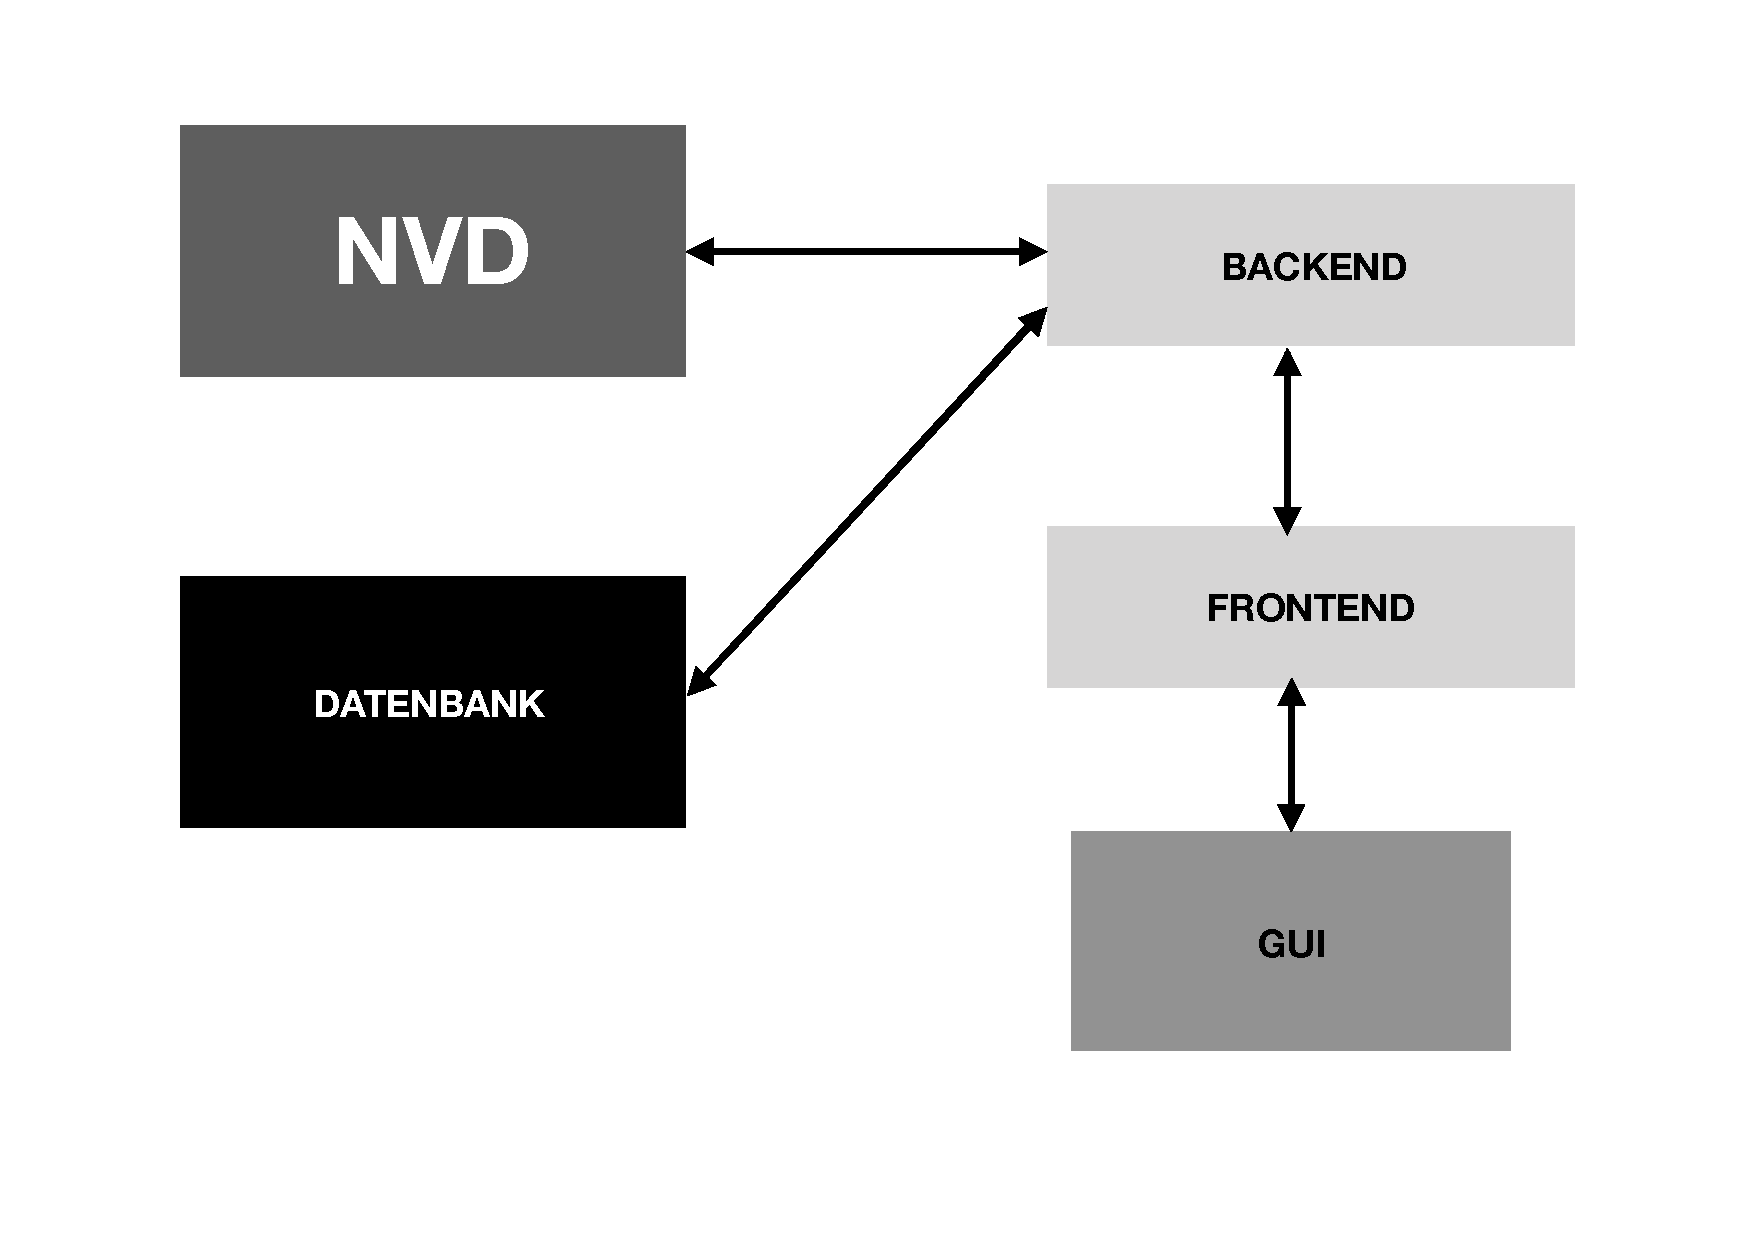
\includegraphics[scale=0.4]{figures/model.pdf}
    \caption{High-Level-Design: Model-View-Controller Modell}
\end{figure}
\\
Des Weiteren wird Spring MVC als Web Framework genutzt, mit dem schnell und einfach eine REST-konforme Webapplikation aufgesetzt werden kann und unter Anderem Dependency Injection ermöglicht wird \cite{johnson2004expert}. 
\section{Planung}
Die zur Verfügung stehenden 11 Wochen werden in 4 große Blöcke eingeteilt. 
Am Anfang des Projektes steht eine Woche, die ganz dem Brainstorming und der Reuqirementanalyse gewidmet ist. Hierbei sollen mögliche Frameworks und Tools, und mögliche Herangehensweisen in Betracht gezogen werden. Daraufhin folgt eine weitere Woche, die der Konzeption und der Entwicklung eines genauen Entwurfs dienen. Eine gute und detaillierte Planung von Back- und Frontend soll eine reibungslose Implementierung ermöglichen und Verzögerungen im weiteren Verlauf des Projekts verhindern. Nun stehen einige Tage zur Einrichtung zur Verfügung. Aufgrund von vier verschiedenen Betriebssystemen ist es wichtig dafür zu sorgen, dass alle auf dem gleichen Stand sind und miteinander interagieren können, z.B. via Git. Die nächsten Wochen dienen der Erstellung eines ersten Prototyps mit einer lokale Datenbank, die mit NVD \cite{nvd} Daten gespeist wird und einer ersten einfache Suche. Wenn diese Grundfunktionalitäten stehen, geht es um die Fertigstellung von Back- und Frontend mittels CI und CD. 
\\
Zur Umsetzung und schnelleren Implementierung wird das Team in zwei Arbeitsgruppen unterteilt – ein Expertenteam für Front- und eins für Backend. Durch wöchentliche Meetings und eine regelmäßige Kommunikation via Slack und Telegram ist die Abstimmung und Synchronisierung der Schnittstellen problemlos. Die letzte Woche vor Abschluss des Projekts soll Zeit einräumen, die fertige GUI, die Suche und Feinheiten zu testen, und entsprechende Tests zu schreiben. \\\\
\begin{figure}[htb]
    \centering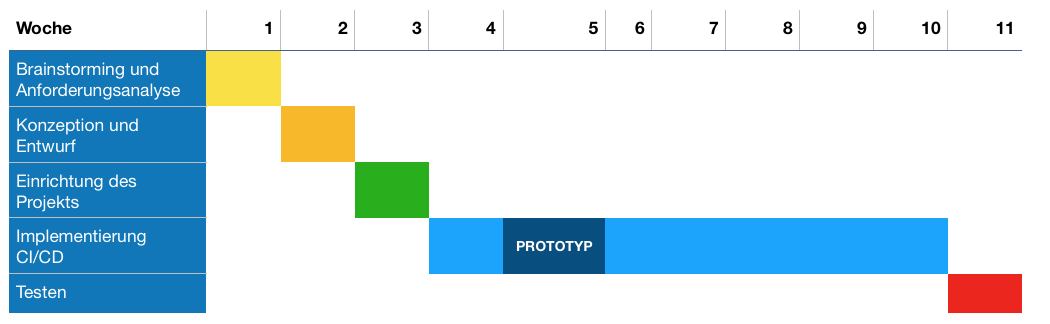
\includegraphics[scale=0.82]{figures/GANTT3}
    \caption{Gantt-Diagramm}
\end{figure}
\chapter{Implementierung (Filip)}

\section{Backend}
Das Backend wurde mit der Hilfe von Spring Framework erstellt. Der Webserver stellt dem Benutzer die entsprechenden Daten zur Verfügung. Außerdem realisiert er die Kommunikation mit der Datenbank, verschiedene  Such verfahren als auch das Herunterladen und Einspeisen der neuen Daten in die Datenbank. Diese Funktionalitäten wurden in vier Klassen implementiert.\\

\textit{Application} ist verantwortlich für den Start des Servers und falls eine entsprechend Flag übergeben wurde, für das Herunterladen und Einspeisen des neuen Datensatzes. Dieses kann auch optional  als automatische Tätigkeit, die in festen Zeitintervallen geplant ist, implementiert werden. In dieser Implementierung wurde es jedoch auf die manuelle, Flag-gesteuerte Weise implementiert.\\

\textit{MongoDBImport} ist eine Klasse, die den eigentlichen Arbeitsablauf bei dem Herunterladen und Einspeisen der neuen Datensätze implementiert. Der neueste Feed wird zuerst heruntergeladen. Danach wird er entpackt und mit Hilfe eines externen Python Skripts entsprechend formatiert, damit die Daten vollständig von der Datenbank gelesen werden können. Schließlich werden die Daten mittels Ausführung der Update-Funktion in die Datenbank eingelesen.\\

\textit{SearchController} ist zuständig für die Behandlung von Views und API Anfragen. Dabei sind die zwei API POST Anfragen, \textit{search/submit} und \textit{search/page}, von entscheidender Bedeutung. Sie sind verantwortlich für die Ausführung der Suchanfrage und für die Berechnung der resultierenden Daten auf der Backend-Seite. Eine derartige Teilung der Funktionalität realisiert Pagination auf der Backend-Seite. Auf diese Weise können bestimmte Teile der Ergebnisse auf Nachfrage nachgeliefert werden.\\

\textit{SearchMethods} realisiert vor allem die Verbindung mit der Datenbank und die eigentlichen Suchverfahren - den Kern der Funktionalität der Applikation. Die Suchen nach CVE, CPE, CWE, CVSS und die Textsuche werden zuerst als einzelne Anfragen generiert und erst vor der Ausführung in der Datenbank verundet. Diese Lösung resultiert in einer intuitiver Suche aus der Sicht des Benutzers, bei der er mit weiteren Kriterien die Anzahl der Ergebnisse flexibel begrenzen kann. Außerdem führt die Klasse eine Möglichkeit ein zwischen einer lokalen und und externen Datenbank zu unterscheiden. Während der Entwicklung wurde ausschließlich eine lokale Datenbank verwendet, in der Testphase jedoch wurde auch eine externe Datenbank benutzt, um die Leistung zu testen.\\

\begin{java}
public class Application {
    public static void main(String[] args);
}
public class MongoDBImport {
    public static void downloadJSON();
    public static void copy(InputStream input, OutputStream output, int bufferSize);
    public static void unzip(String zipfile);
    public static void mongoImport();
}
public class SearchController implements WebMvcConfigurer {
    public void addViewControllers(ViewControllerRegistry registry);
    public JSONObject searchSubmit(@RequestParam Map<String, String> params);
    public JSONObject searchPages(@RequestParam Map<String, String> params);
}
public class SearchMethods {
    public static void setLocalDatabaseFlag();
    public static boolean getLocalDatabaseFlag();
    public static void dbConnect();
    public static JSONObject mainSearch(Map<String, String> params);
    public static JSONObject getPage(Map<String, String> params);
}
\end{java}

\section{Frontend}
Auf der Clientseite hat sich das Team dazu entschlossen, eine Webpräsenz als Single Page Application zu implementieren. Die Seite besteht aus einer HTML und einer CSS Datei, in der die Struktur und der statische Teil der Darstellung definiert sind und aus einer Javascript Datei, die die ganze Funktionalität der Seite realisiert.\\

% HTML & CSS - Struktur der Webseite
Die Struktur der Webseite besteht aus drei Inhaltsbereichen. Links angeordnet ist ein  Menü mit Referenzen auf  statische Unterseiten, die die Dokumentation sowohl der API als auch des Projektes als Ganzes beinhalten. Unter den Referenzen befindet sich das Formular für die Suchanfrage mit dem direkt in HTML als \textit{pattern} Attribut verfügbaren  Validierungsverfahren. Die Ergebnisse einer Suchanfrage erscheinen in dem rechts angeordneten Inhaltsbereich. \\

% JS - Verhalten der Webseite 
Die Webseite realisiert folgende Funktionen: dynamisches Umschalten der Unterseiten, Aufnehmen der Suchanfragen, Kommunikation mit dem Server mittels API und geeignete Darstellung der Ergebnisse mit Pagination. Sowohl das Umschalten, Annehmen der Suchanfragen als auch die Kommunikation mittels API wurden mit der Hilfe von \textit{event listeners} und \textit{ajax requests} aus der \textit{jQuery} Bibliothek umgesetzt. Die empfangene Ergebnisse beinhalten immer die ganzen Datensätze, deshalb sind die Parserfunktionen von zentraler Bedeutung um nur die relevante Attribute zu extrahieren. Die  Funktionen verfolgen das Bennenungsschema \textit{get$\langle$NameOfAttribute$\rangle$} und die grobe Struktur: Behandlung der Randfälle wie beispielsweise Nullwerte. Alle geben auch eine HTML-Zeichenkette zurück, die direkt als Inhalt einer Tabellenzelle hinzugefügt werden kann. Die Parserfunktionen werden von der Überfunktion benutzt, die für die Kommunikation mit dem Server, Erstellung der Metriken und Generierung der Tabelle mit Ergebnissen zuständig ist. Die Tabelle zeigt die wichtigsten Attribute der Datensätze (CVE, Vendors, Description, CPE, CVSS Score) sofort als sichtbaren Inhalt. Weitere Informationen zum jeweiligen Datensatz, können durch den erweiterbarer Tabelleneintrag abgerufen werden.\\

\section{Tests}
Ausgewählte Kernfunktionen sowohl von dem Server als auch von der Webseite wurden mittels Unit Tests auf Korrektheit geprüft. Mit der Hilfe von \textit{JUnit} Tests \cite{Massol2004JUnitAction} wurde getestet, ob das Herunterladen und das Entpacken der JSON Dateien fehlerfrei abläuft. \textit{Jest} Javascript Bibliothek wurde verwendet, um die Korrektheit des Inhalts und der Darstellungsform der einzelnen extrahierten Informationen zu prüfen \cite{Banker:2011:MA:2207997}.


\chapter{Evaluation (Patrick)}

    Zu Beginn des Projektes hat das Team sich dazu entschlossen das Java-Framework JHipster zu benutzen \cite{JHipsterApplications}. In Verbindung mit einem Klassendiagramm, passend zu der Datenstruktur der NVD Datenbank, sollten die Daten der National Vulnerability Database (NVD)\cite{nvd}, in eine relationale Datenbank gespeichert werden. Aufgrund der Unverhältnismäßigkeit zwischen Aufwand und Nutzen ergab eine erneute Evaluation, dass das Projekt mit dem Spring Framework und noSQL (MongoDB \cite{mongodb}) einfacher und effektiver umgesetzt werden kann. Diese Entscheidung ermöglichte ein effektiveres und produktiveres Arbeiten mit klar abgegrenzten Aufgaben (SCRUM). Mehrere Methoden wie z.B.: Feedback Gespräche, Reviews und Sprint Planungen ermöglichten eine effiziente Bearbeitung der Anforderungen. 
    \\

    Das Resultat des Projektes ist eine Webapplikation in der nach Software-Schwachstellen, die in der NVD gelistet sind, gesucht werden kann. Die Ergebnisse der Suche werden in einer Liste mit aufklappbaren Elementen dargestellt. Eine farbliche Markierung, angelehnt an das \glqq Common Vulnerability Scoring System\grqq{} (CVSS) bietet eine Unterscheidung der Ergebnisse nach Ihrer \glqq Schwere\grqq{} \cite{CommonSIG}. 
    Die so entstandene Plattform, siehe Abb. A.1, ermöglicht einen schnellen und übersichtlichen Zugriff auf die Daten der NVD.
    Die Umsetzung der Suche mit Regex ermöglicht eine anpassbare Applikation, die mit geringen Modifikationen verschiedene Suchmöglichkeiten bietet. MongoDB in Verbindung mit noSQL speichert zwar redundante Daten wie Beispielsweise den Hersteller, jedoch haben alle (manuell) getesteten Suchanfragen in angemessener Zeit Resultate geliefert. Die Umsetzung der 'Datenstruktur' erforderte kein aufwändiges relationales Datenmodell wie es beispielsweise bei Nutzung mit SQL der Fall wäre. Da jedes Datenbank update durchschnittlich 8-12 MegaByte groß ist, ist eine Umsetzung mit noSQL kein Problem. 
    \\
    
    Die Anwendung der SCRUM-Methode für die Realisierung des Projektes hat in der frühen Projektphase dazu geführt, dass wir von JHipster zu einem Spring Projekt gewechselt haben \cite{Rising2000TheTeams}. Dieser Wechsel beschleunigte das Erreichen der Meilensteine um ein vielfaches, sodass das Projekt zügig, mit allen Anforderungen realisiert werden konnte.
    \newpage
\chapter{Fazit und Ausblick (Patrick)}
    
    % https://link.springer.com/chapter/10.1007/978-3-642-23088-2_15
    Aufgrund der klar formulierten und ausführlichen Anforderungen gestaltete sich die Analyse der Anforderungen und die Umsetzung des Projektes ohne Probleme. Die Erfahrung, die mit JHipster gesammelt wurde, konnte zügig mit Spring umgesetzt werden, sodass mit Hilfe von \glqq Model View Control \grqq{} eine funktionale Applikation entwickelt werden konnte.
    \\
    
    Sowohl die Einteilung der Arbeitspakete, als auch die zeitliche Planung führten zu einem Resultat, welches die Anforderungen vollständig erfüllt. Durch wöchentliche Treffen und die Einhaltung von SCRUM, verbesserten sich die Absprachen und die Zusammenarbeit. Sämtliche Aufgaben wurden in geplanter Zeit erledigt und Entscheidungen in gemeinsamer Abstimmung getroffen. Aufgrund der guten Zusammenarbeit, welche gegenseitige Kritik, Anmerkungen, Feedback und Verbesserungsvorschläge beinhaltet, sind auch weiterführende Projekte denkbar. Beispielsweise die Verwendung der Suche über eine REST Schnittstelle für einen Vergleich zwischen einer Software-Datenbank und der NVD-Datenbank. Ein Vergleich könnte Schwachstellen bestehender System entdecken und mit Warnungen auf Updates für mehr Sicherheit in IT-Systemen hinweisen. 
    \\  
    
    Für zukünftige Projekte wie z.B. das Projekt von Rainer Bye et. al.\cite{bye:2010:CollSec} kann die Applikation genutzt werden um vorhandene Software-/Hardware Komponenten in IT-Netzwerken zu analysieren und mit aktuellen Einträgen aus der NVD zu vergleichen.
    Ein solcher Vergleich der Einträge kann dabei automatisiert werden, beispielsweise mit Nagios\cite{Nagios}, einer IT Infrastruktur Monitoring Applikation. Mit dieser Applikation können Benachrichtigungen und Warnungen eingerichtet werden um vor eventuellen Gefahren gewarnt werden und schaden abgewendet.


\bibliographystyle{abbrvdin}
%\addcontentsline{toc}{chapter}{Literatur}
\bibliography{bib_manual_all.bib}

%%%%%%%%%%%%%%%%%%%%%%%%%%%%%%%%%%%%%%%%%%%%%%%%%%%%%%%%%%%%%%%%%%%%%%%%%%%%
% Appendix remove if none
%%%%%%%%%%%%%%%%%%%%%%%%%%%%%%%%%%%%%%%%%%%%%%%%%%%%%%%%%%%%%%%%%%%%%%%%%%%%
\appendix
\chapter{Anhang}
\begin{figure}[htb]
    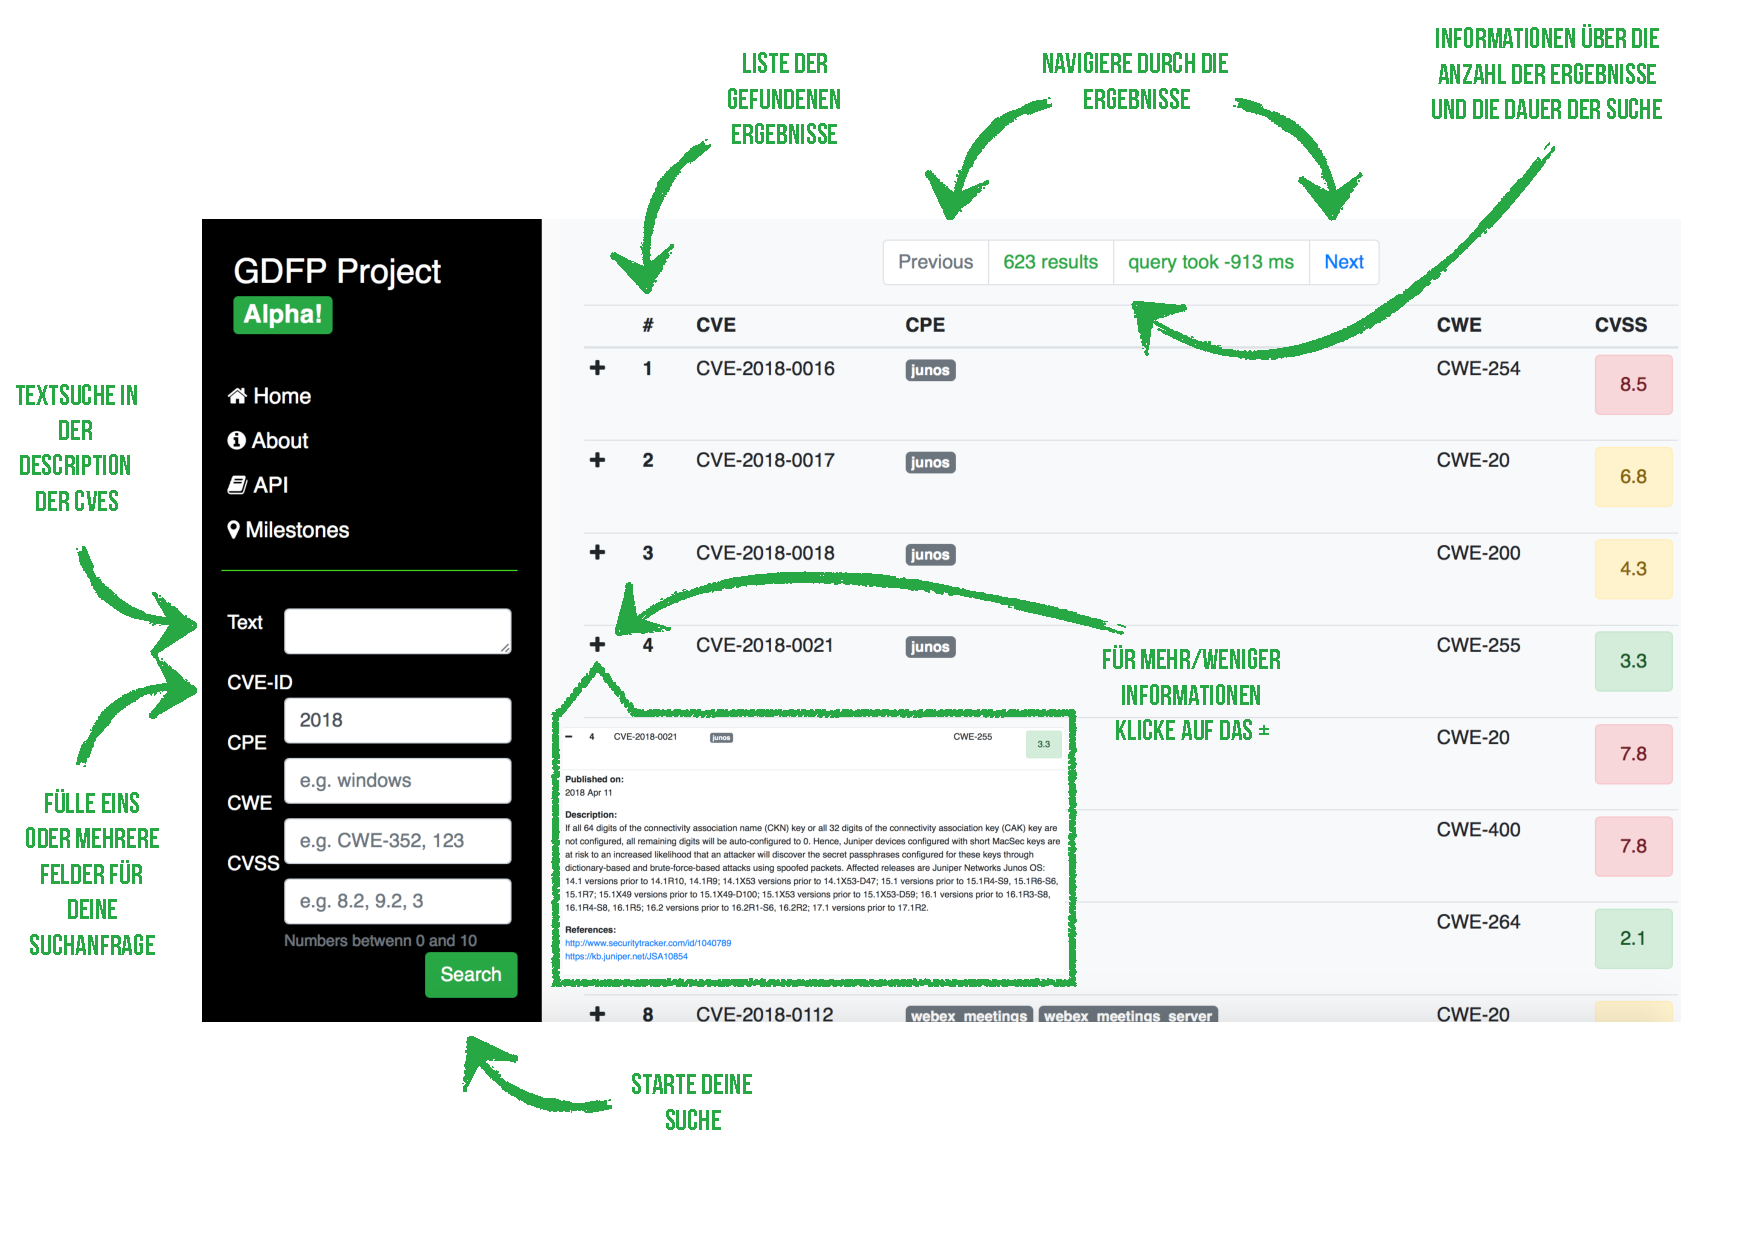
\includegraphics[width=1.1\textwidth]{figures/about_page1.pdf}
    \caption{Beschrifteter Screenshot der Benutzeroberfläche}
\end{figure}

%%%%%%%%%%%%%%%%%%%%%%%%%%%%%%%%%%%%%%%%%%%%%%%%%%%%%%%%%%%%%%%%%%%%%%%%%%%%
\end{document}
